\documentclass[10pt,journal,finalsubmission,compsoc]{IEEEtran}

% *** CITATION PACKAGES ***
%
\ifCLASSOPTIONcompsoc
  % IEEE Computer Society needs nocompress option
  % requires cite.sty v4.0 or later (November 2003)
 \usepackage[nocompress]{cite}
\else
  % normal IEEE
  % \usepackage{cite}
\fi

\setlength{\textfloatsep}{3pt plus 1pt minus 0.5pt}

%\usepackage{appendix}
\usepackage{amssymb}
\usepackage{algorithm}
%\usepackage[noend]{algorithmic}
\usepackage{amsmath}
\usepackage{amssymb}
\usepackage{array}
\usepackage{graphicx}
\usepackage{pifont}
\usepackage{epsfig,tabularx,amssymb,amsmath,subfigure,multirow,booktabs}
\usepackage{balance}
\usepackage{bm}
%\usepackage[noend]{algpseudocode}
\usepackage{algpseudocode}
\usepackage{epsfig,subfigure}
\usepackage{mathptmx}
\usepackage{url}
\usepackage[marginal]{footmisc}


\begin{document}

\title{Accelerate Distributed Stochastic Gradient Descent with Asynchronous Communication Protocol}

\author{Yuewei~Ming,
Yawei~Zhao,
Deke~Guo~\IEEEmembership{Member,~IEEE,}
Jianping~Yin
\IEEEcompsocitemizethanks
{\IEEEcompsocthanksitem Y. Zhao, Y. Ming, and J. Yin are with the College of Computer, National University of Defense Technology, Changsha 410073, P.R. China. E-mail: \{zhaoyawei09, jpyin\}@nudt.edu.cn, and myw123@163.com.
\IEEEcompsocthanksitem D. Guo is with the Science and Technology on Information System Engineering Laboratory, National University of Defense Technology, Changsha 410073, P.R. China. E-mail: guodeke@gmail.com.%\IEEEcompsocthanksitem J. Xu is with the School of Computer, Electronics and Information, Guangxi University, Nanning 530004, P.R. China. E-mail: xujia@gxu.edu.cn.
}
}
\IEEEcompsoctitleabstractindextext{%
\begin{abstract}
Asynchronous and distributed Stochastic Gradient Descent (SGD) with the variance reduction technique such as Stochastic Variance Reduction Gradient (SVRG) has been proved powerful to train various machine learning tasks. However, it cannot support the distributed machine learning algorithms directly because of excessive volume of training data in the era of Big Data. Although conventional work such as PetuumSGD performs well for distributed machine learning tasks, they focus on the optimization on communication protocols for iterative convergence algorithms which do not exploit the potential benefit of a specific machine learning algorithm. We analyze both SVRG and the asynchronous communication protocol in PetuumSGD, and propose a distributed implementation of SVRG by combining both of them together. Furthermore, we optimize our distributed SVRG with many tricks including an accelerated factor for the constant learning rate and adaptive sampling strategy to exploit the benefits SVRG. Extensive empirical study verifies that our distributed SVRG  performs better on accelerating iterative convergence machine learning algorithms than pioneering work such as PetuumSGD. 
\end{abstract}

\begin{IEEEkeywords}
Stochastic gradient descent, Staleness synchronous protocol, Distributed machine learning algorithms.
\end{IEEEkeywords}}

\maketitle

\IEEEpeerreviewmaketitle

\section{Introduction}
\label{introduction}






\section{Related work}
\label{related_work}




\subsection{Asynchronous distributed stochastic gradient descent}





\section{Preliminaries and Overview}
\label{overview}
Many machine learning algorithms can be described by using 

\begin{equation}
\label{equa_loss_minimization}
\begin{split}
 & \min F(w) \\
 & F(w)=\frac{1}{n}\sum\limits_{i=1}^n f_i(w)\\
\end{split}
\end{equation}.

Here, $n$ means the size of training data, and $w$ represents the parameters of a machine learning model, that is, the parameters needed to be updated during the iterations. Conventionally, each $f_i(w)$ is a $L$-smooth function so that $\exists$ a non-negative $L$, and $\forall$ $a$ and $b$, the following inequality holds.

\begin{equation}
\label{equa_l_smooth} 
f_i(a)\le f_i(b)+\nabla f_i(b)^\mathrm{T} (a-b)+\frac{L}{2}\parallel a-b\parallel^2
 \end{equation}.
 
The inequality can be described equivalently as follows.

\begin{equation}
\label{equa_l_smooth2} 
\parallel f_i(a)-f_i(b)\parallel^2\le L \parallel a-b\parallel^2
 \end{equation}
 or $\exists$ a non-negative $C$, the following inequality holds.
 
 \begin{equation}
\label{equa_l_smooth3} 
\parallel \nabla f_i(a)-\nabla f_i(b)\parallel\le C
 \end{equation}


Besides, the loss function $F(w)$ is $\gamma$-strongly convex, which means that $\exists$ a non-negative $\gamma$, and $\forall$ $a$ and $b$, the following inequality holds.

\begin{equation}
\label{equa_gamma_convex} 
F(a)\ge F(b)+\nabla F(b)^\mathrm{T} (a-b)+\frac{\gamma}{2}\parallel a-b\parallel^2
\end{equation}.

The inequality can be presented equivalently as follows.

\begin{equation}
\label{equa_gamma_convex} 
\parallel F(a)-F(b)\parallel \ge \gamma \parallel a-b\parallel
\end{equation}.

Many machine learning algorithms can be represented by this abstraction including regression and classification and so forth. 

 
Inspired by the variance reduction in \cite{Johnson:9MAvkbgy}, we present the overview of our asynchronous and distributed SGD in Algorithm \ref{algorithm_dis_svrg}. Our asynchronous and distributed SGD consists of three ingredients: epochs of iterations (the outer for loop at Line 2), random update strategy of parameters (the inner for loop at Line 6) and update rule of parameters (Line 8 and 9). We abstract all the threads running on machines of a cluster as two ingredients: the servers and the trainers. The epochs of iterations is conducted by the servers which adopts asynchronous communication protocol, i.e., SSP to proceed the iterations for all trainers. The random update strategy of parameters is conducted by the trainers which randomly pick one of $n$ candidate training samples, compute the variance reduced gradient, and then update such gradient to parameters. 

\begin{algorithm}[t]
    \caption{DisSVRG}
    \label{algorithm_dis_svrg}
    \begin{algorithmic}[1]
        \State Initialize $\tilde{\omega}^0$
        \For {$s=1,2,...$} \% Asynchronous learning parameters for all trainers
            \State $\tilde{\omega}=\tilde{\omega}^{s-1}$
            \State $\mu=\frac{1}{n}\sum\limits_{i=1}^n\nabla f_i(w_i)$
            \State $\omega_0=\tilde{\omega}$
            \For {$t=1,2,...m$} \% Variance reduction technique used in each trainer 
                \State randomly pick $i_t\in\{0,1,2,...,m\}$
                \State $v_t=\nabla f_{i_t}(w_{t-1})-\nabla f_{i_t}(\tilde{\omega})+\mu$ \% stochastic variance  reduced gradient
                \State $w_t=w_{t-1}-\eta v_t$
           \EndFor
           \State $\tilde{w}_s=w_m$
       \EndFor
    \end{algorithmic}
\end{algorithm}

A global state of parameters is maintained by all servers. When the iteration begins, all trainers pull the global parameters from one of servers. Then all the trainers start to conduct the machine learning tasks asynchronously. To be specific, each a trainer computes the variance reduced gradients and update its local copy of global parameters.   When a trainer finish to update its local parameters, it will push its local copy of parameters to one of servers. Since the runtime environment of machines are various, the computation time of variance reduced gradient  is not same. However, the fast trainers will continue to proceed the iterations, and  not wait the slow ones. On the other hand, the asynchronous SGD may not converge if all the trainers update parameters in a fully asynchronous way. Here, we set a delay bounded, i.e., $\tau$. The delay $\tau$ is used to synchronize all the trainers. Specifically, when the fastest trainer finishes the $t$th iteration, and the slowest trainer does not finish the $(t-\tau)$th iteration,  it will be forced to stop and wait the slowest trainer. 

\section{System implementation}
\label{implementation}
DisSVRG is implemented by the servers and trainers where the servers maintain the local state of parameters, and the trainers compute the updates of parameters. The servers receive the updates of parameters from trainers, and then aggregate these updates into the local parameters. Each a trainer pushes a copy of a global parameters before it starts to conduct machine learning tasks. When a trainer finishes the updates of parameters during an epoch, it will pull the latest local parameters to one of servers. If a trainer has finished the $t$th epochs, and all the trainers have finished the $t-\tau$th epochs, then this trainer will pull the aggregated parameters and starts to another epoch, or it will have to wait. To be specific, the details of DisSVRG are presented as follows.

\textbf{Server:} 



\begin{algorithm}[t]
    \caption{Server}
    \label{algorithm_dis_svrg_server}
    \begin{algorithmic}[1]
        \State Initialize $\tilde{\omega}^0$
        \While {true}
            \If {receive a pull request from the trainer $p$}
                \State $e_p=p.epoch$
                \If {other trainers have finished $e_p-\tau$th epoch}
                    \State send a copy of the global parameters.
                \EndIf
            \EndIf
            \If {receive a push request from the trainer $p$}
                \State receive the parameters from the trainer $p$, and aggregate them with the local parameters.
            \EndIf
        \EndWhile
    \end{algorithmic}
\end{algorithm}




\textbf{Trainer:}



 
\begin{algorithm}[t]
    \caption{Trainer}
    \label{algorithm_dis_svrg_trainer}
    \begin{algorithmic}[1]
        \State $e_p=0.$
        \While{true}
            \State send a pull request to a server
            \While {true}
                \If {receive a copy of global parameters from the server}
                    \State $e_p=e_p+1.$
                    \For {$t=0,1,2,..., m$}
                       \State random pick a non-negative number $i$ with $i\in\{0,1,.2,...,n\}$
	              \State $v_t=\nabla f_{i_t}(w_{t-1})-\nabla f_{i_t}(\tilde{\omega})+\mu$ 
	              \State $w_t=w_{t-1}-\eta v_t$ 
                    \EndFor
                    \State send the latest parameter $w_m$ to a server.
                 \EndIf 
        \EndWhile
      \EndWhile
    \end{algorithmic}
\end{algorithm}







\section{Optimization of asynchronous and distributed SGD}
\label{optimization_sgd}
In this section, we present two optimization tricks which can be used to accelerate DisSVRG in a cluster. 

\subsection{Learning rate with accelerated factor}
Generally, variance reduction technique accelerates machine learning algorithms by using a constant learning rate. Even though the constant learning rate performs well for $L$-smooth and $\gamma$-strongly convex objection function, some inner properties can be exploited to accelerate the convergence of the machine learning algorithms. 

Based on the inequality \ref{equa_l_smooth3}, when $b$ is valued the optimal weight, i.e., $w^\ast$, $\forall$ $w$, it holds that $\parallel\nabla f_i(w)\parallel \le C$. That is, when the parameters are updated, the absolute value of the gradient is bounded by a constant. Besides, the gradient of parameters decreases when such parameters approach to the optimal state. Especially, when the parameters are close to  the optimal state, their gradient reaches zero approximately. Therefore, we introduce an accelerated factor $\sigma$ with $\sigma=\parallel \nabla f_i(w)\parallel$. The learning rate of our SGD contains two ingredients: the constant and the accelerated factor. The constant part of DisSGD prevalents  it to get struck at the local optimal state; while the accelerated factor makes DisSGD converge at a more than constant rate. Furthermore, since the gradient of  each function $f_i(w)$ has an upper bound, the accelerated factor do not become very large and lead to the divergence of the objection. 

As illustrated in Fig. \ref{figure_evaluation_accelerated_factor}, we deploy such an accelerated factor in linear regression tasks. Here, the evaluation test is conducted on a machine instead of a cluster. The dataset is \emph{YearPredictMSD} which is the biggest dataset we can find to conduct linear regression tasks. The settings of this evaluation test  is and more evaluations are presented in Section \label{performance_evaluation}. 
The solid lines represent the machine learning task with the basic learning rate $\eta \mathrm{=}0.001$; while the dotted lines stands for the machine learning task with the basic learning rate $\eta \mathrm{=}0.01$. Additionally, the blue lines means that the machine learning algorithm is trained by using a constant learning rate, but the red lines means that such machine learning algorithm is trained by using an incremental learning rate. The incremental learning rate consists of a basic learning rate and a accelerated factor. We can get two important observations from Fig. \ref{figure_evaluation_accelerated_factor}. First, the learning rate with an accelerated factor makes the machine learning algorithm converges faster than the learning rate without such a accelerated factor. Second, such benefits due to the accelerated factor becomes large when the basic learning rate increases. Shortly,  the accelerated factor gives rise to obvious benefits for the machine learning algorithms.

\begin{figure}
\centering
\subfigure{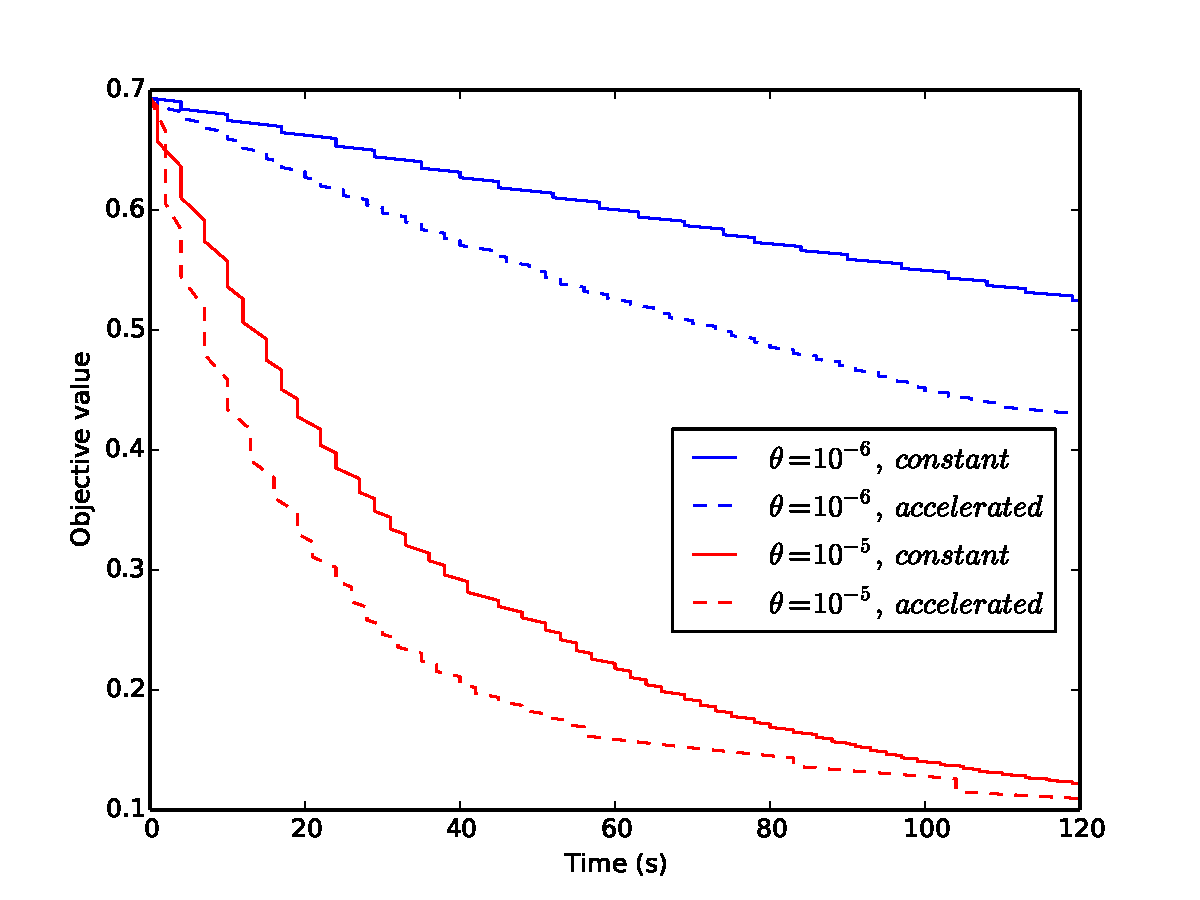
\includegraphics[width=0.86\columnwidth]{figures/evaluation_accelerated_factor}}
\caption{DisSVRG with the accelerated factor converges faster than DisSVRG.}
\label{figure_evaluation_accelerated_factor}
\end{figure}



\subsection{Adaptive strategy of the random updates}

Since DisSVRG needs the strategy of random updates in its inner loop, it is important to identify how many random updates in an epoch is appropriate to achieve a good tradeoff between time and accuracy.  As illustrated in the inner loop of Algorithm \ref{algorithm_dis_svrg}, $m$ represents the number of random updates for an epoch. First, $m$ cannot be given a large number such as $O(n)$. Here, $n$ means the size of the training data.  In order to maintain a satisfied accuracy, DisSVRG have to conduct the inner loop serval times, which consumes much time since the training data becomes extremely huge such as millions or billions of samples. Especially, we can get billions or trillions of samples from sensors in the world or Internet, a large $m$ like $O(n)$ makes the runtime of DisSVRG unacceptable.  On the other hand, $m$ cannot be set a small value straightly.    To gain a high accuracy of the objection function, a small $m$ leads to many epochs of DisSVRG. However, an average gradient is needed for  an epoch, which leads to $n$ deprivation operations. Therefore, a small $m$ costs too much time due to the deprivation operations. As illustrated in Fig. \ref{figure_evaluation_random_strategy}, we conduct an evaluation test on a  machine by varying the value of $m$. Here, the dataset is still \emph{YearPredictMSD}, and the learning rate, i.e., $\theta$ is set to a constant with $\theta=10^{-5}$. It is obvious that a large $m$ brings a fast convergence of the objective function because such a large value of $m$ gets rid of frequent computation of the average gradient.

Additionally, a cluster such as EC2 is often heterogenous so that machines in the clusters perform differently due to the diversity of the hardware. Intuitively, some machines in the cluster conduct DisSVRG  fast; while others perform DisSVRG slowly.  Therefore, it is suitable and practical that the number of inner loops of DisSVRG, i.e., $m$, should be flexible to be adjusted for each a machine. In other words, DisSVRG should allow that $m$ on different machines can be set a different value. Intuitively, the machines which run fast should have a larger $m$ than the machines which run slow. Although the staleness synchronous protocol, i.e., SSP, allows a delay bound for such those machines which runs slow, those machines running fast have to wait the machines running slow until the delay is achieved.  This is usually called the ''the straggler problem'.  

We adopt an adaptive strategy of the random updates which dynamically adjust $m$ in order to reduce the waiting time caused by the straggler problem. When an epoch, e.g., $t$, of DisSVRG is completed, the updated parameters on the local machine will be pushed to a server. If the delay bound is denoted by $\tau$, the server will check the epochs of other machines. If there exists at least one machine which has not finished the $t-\frac{\tau}{2}$ epoch, then the fast machine increases its number of the inner loop, i.e., $m$, to $m+\delta$. Here, $\delta$ is a constant non-negative integer. By using this adaptive strategy, the fast machines will spend more time on computing the updates of parameters than the slow machines, which not only reduces the waiting time caused by the straggler problem, but also improves the convergency of DisSVRG. 


\begin{figure}
\centering
\subfigure{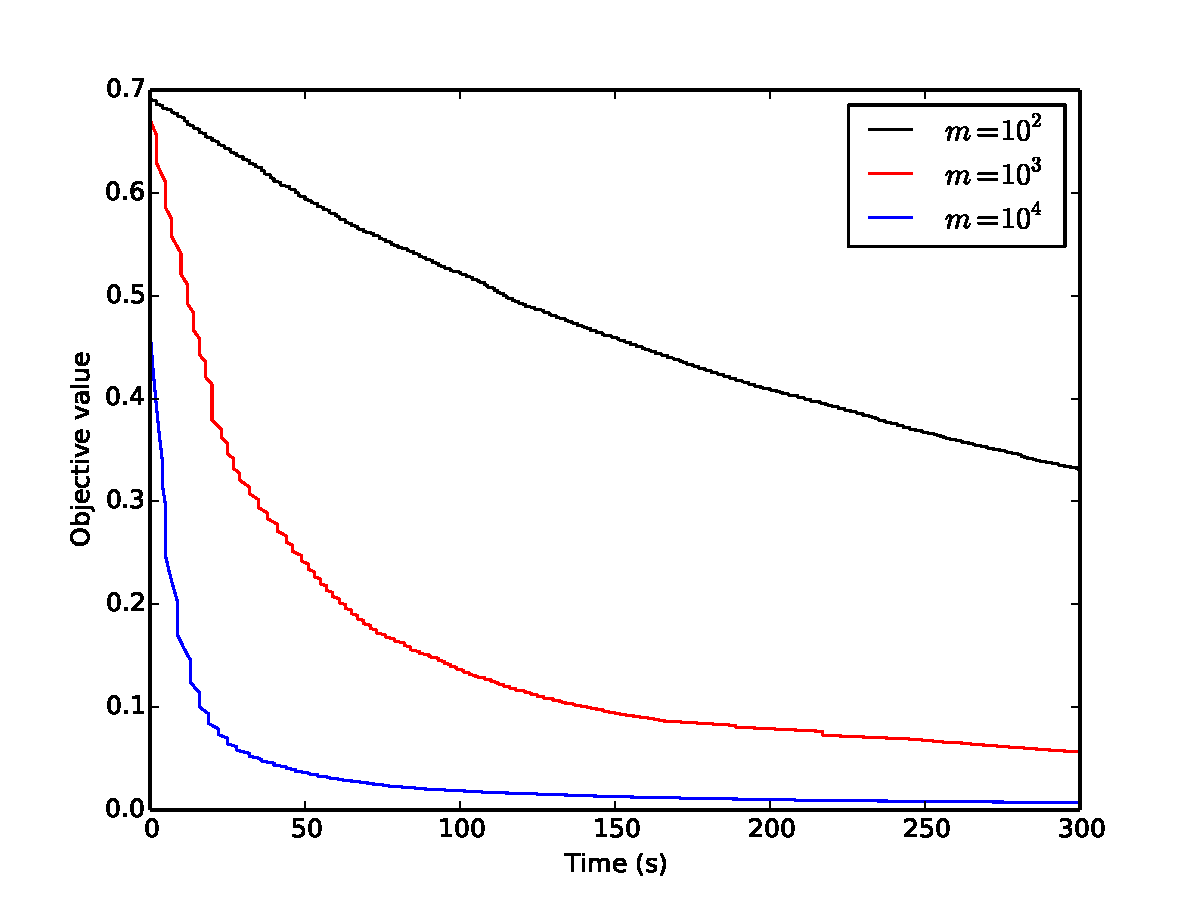
\includegraphics[width=0.86\columnwidth]{figures/evaluation_random_strategy}}
\caption{A large $m$ leads to a fast convergence for DisSVRG.}
\label{figure_evaluation_random_strategy}
\end{figure}




\section{Discussion}
\label{discussion}
The machine learning tasks such as Deep learning are generally fed with extremely large volume of training data in the era of Big Data. However, conventional serial variants of SGD  cannot consume training data on a single machine within the available time. Although distributed variants of SGD such as PetuumSGD are designed to solve this challenge, those existing SGD versions are always presented as demos of some distributed machine learning systems like Petuum. SGD has its inner weakness such as the variance due to the random update of parameters. Such those distributed machine learning systems thus decrease the learning rate to reduce the variance, which leads to slow convergence of SGD. The main reason is that when machine learning tasks are proceeded, the learning rate will be decreased to a very small value so that every iteration bring tiny benefits to the loss function. Even though existing distributed machine learning systems have made much optimization on the communication mechanism, SGDs embedded on those systems are not exploited to accelerate machine learning tasks. 

We do not aim to proposing another a general platform for distributed machine learning algorithms, but focus on the optimization of SGD in a distributed system. Our implementation of distributed SGD adopts SSP as the consistency protocol which is suitable to iterative convergence machine learning algorithms. The most difference between our implementation of distributed SGD between PetummSGD is the variance technique adopted in the algorithm. PetuumSGD adopts standard SGD with the decreasing learning rate $O(\frac{1}{\sqrt{T}})$. Here, $T$ means the epochs of iterations. Variance of PetuumSGD will be decreased when the learning rate becomes small. However, our implementation of SGD has been accelerated with two ingredients: the constant factor and the accelerated factor. The constant factor makes sure that our SGD keep a constant rate to reach to the optimal value. The accelerated factor will make the machine learning algorithm converge fast. Even though our SGD adopts the same consistency protocol with PetuumSGD, our SGD trains parameters at a faster rate than PetuumSGD by using a powerful variance technique. 

Comparing with SVRG, our SGD is a asynchronous and distributed version. In the era of Big Data, the size of training data is extremely huge so that a single machine cannot handle all the training data. Since the service of data center is trivial to use,  it is natural to perform machine learning algorithms with a cluster, instead of an machine. Inspired by the variance reduction technique of SVRG, we implement a new distributed SGD. Our SGD is different from SVRG with at least three aspects. First, we extend the serial SVRG to an asynchronous and distributed version by using the asynchronous consistency protocol, i.e., SSP. Second, comparing with the constant learning rate in SVRG, the learning rate in our SGD contains an accelerating factor which exploits the potential benefits of the loss function and make the machine learning algorithms converge fast. Third, the variance reduction of SVRG needs at most $m$ random updates of parameters. $m$ is valued as the times of the size of training data, which is not practical for a large volume of training data. Our SGD achieve the value of $m$ by maintaining a window of the value of loss function and then analyzing them dynamically. Such an identification of $m$ is suitable to the practical scenarios because that each learning thread can have its own setting of $m$.  The reason is that the machines in the cluster may be very heterogeneous, and the learning threads are not synchronized during an epoch of iteration. The adaptive mechianism of the value of $m$ is suitable to such situations.

Additionally, comparing with the SGD in \cite{Zhang:2015tp}, our SGD adopts a more natural way to implement distributed SGD with the variance reduction. SGD in \cite{Zhang:2015tp} implements $\tau$-delay bounded consistency protocol in the inner loop of SVRG; while the epochs of iterations keep fully consistency protocol, namely, BSP. Therefore, SGD in \cite{Zhang:2015tp} has at least two weakness. First, the BSP consistency protocol for the epochs of iterations is not suitable to the iterative convergence machine learning tasks. Since the straggler problem exists in the learning threads due to the variety of system runtime environment, the fast learning threads in SGD in \cite{Zhang:2015tp} have to wait the slow learning ones in an epoch. Considering that machine learning algorithms are iteratively convergent, such BSP consistency protocol wastes too much time. Second, the SGD in \cite{Zhang:2015tp} is coupled with the hardware of clusters. The reason is that SGD in \cite{Zhang:2015tp} uses $m$ learning threads to perform machine learning tasks where $m$ is the number of inner loop in an epoch. $m$ in SGD in \cite{Zhang:2015tp} is valued $O(n)$ where $n$ represents the size of training data. Considering the huge size of training data, $m$ is really large, which is not practical to a  cluster. Instead, $m$ in our SGD is identified by the adaptive and dynamical mechanism, which is flexible to adjust during the calculation of parameters.


\section{Performance evaluation}
\label{performance_evaluation}




\section{Conclusion}
\label{conclusion}


\balance

\ifCLASSOPTIONcompsoc

  \section*{Acknowledgments}
\else

  \section*{Acknowledgment}
\fi
The work is partially supported by the National Natural Science Foundation of China (NSFC) under Grants NO. 61402494, NO. 61402513, NO. 61202487, NO. 61170287, NO. 61232016. Besides, the project is sponsored by the Scientific Research Foundation of GuangXi University under Grant No. XGZ141182.


\bibliographystyle{IEEEtran}
\bibliography{IEEEabrv,reference}


\end{document}

